\chapter{Supporting User Privacy Preferences in Digital Interactions}
\label{ch.privacy_pref}
%Alessandro
%%%%%%%%%%%%%%%%%%%%%%%%%%%%%%%%%%%%%%%%%%%%%%%%

\section{Introduzione}
Per la disponibilità dei servizi online si verifica la situazione in cui il server che fornisce il servizio e l'utente che lo richiede sono ignoti l'uno all'altro.
Di conseguenza sistemi di access control tradizionali non possono essere adottati in quanto non adatti a scenari open.

Soluzioni proposte sono basate su ABAC (Attribute-Based Access Control).
Policy che regolamentano l'accesso ai servizi definiscono condizioni che il client richiedente deve soddisfare per avere accesso.

Il server, a seguito di una richiesta di accesso risponde con le condizioni che il client deve soddisfare per essere autorizzato ad accedere al servizio.

$\\$
Per accedere il client rilascia \textbf{certificati digitali} come \textbf{credenziali} firmate da una \textbf{CA}.
L'adozione delle credenziali nell'Access Control ha diversi vantaggi:
\begin{itemize}
    \item Non serve $<$\textit{username,password}$>$ per ogni servizio.
    \item Offre migliore protezione dall'acquisizione impropria dei privilegi di accesso.
\end{itemize}

$\\$
L'uso di credenziali è stata approfonditamente studiata dal lato server con definizione di diversi \textit{policy languages}, \textit{policy engines} e strategie per la comunicazione delle consizioni di accesso.

Le soluzioni trovate, sebbene potenti ed espressive, non supportano completamente gli specifici criteri di protezione dei client.
Infatti i client necessitano di un sistema di preferenze che permetta di supportare una propria definizione di sensitivity/privacy per i propri dati.
Queste preferenze verranno poi usate nella situazione in cui più di un subset di credenziali soddisfano la Access Control Policy definita dal server.




Questo capitolo mostra una overview delle problematiche di privacy legate ai sistemi open, oltre che alcune soluzioni.
Le sezioni riportano:
\begin{itemize}
    \item Concetti Base e \textit{Desiderata}.
    \item Soluzione Cost-Sensitive Trust Negotiation. 
    \item Soluzione Point-Based Trust Management.
    \item Soluzione Logical-Based Minimal Credential Disclosure.
    \item Soluzione Privacy Preferences in Credential-Based Interactions
\end{itemize}





%%%   %%%   %%%
\section{Concetti Base e \textit{Desiderata}}

\subsection{Client Portfolio}

\begin{definition}[\textit{Client} Portfolio] $\\$
    Insieme delle informazioni che un cliente può fornire al server per avere accesso ad un servizio è racchiuso in un \textbf{Portfolio} contenente \begin{itemize}
        \item \textbf{Credenziali} firmate da third party.
        \item \textbf{Dichiarazioni} che comprendono proprietà non certificate dichiarate dall'utente.
    \end{itemize} 
\end{definition}

\subsubsection{Struttura Credenziale}
Ogni credenziale $c$ è composta da:
\begin{itemize}
    \item Identificatore univoco $id(c)$.
    \item Emittente $issuer(c)$.
    \item Un set di attributi $attributes(c)$.
    \item La tipologia della credenziale $type(c)$.
\end{itemize}


\subsubsection{Gerarchia Tipologie}
I tipi di credenziale sono organizzati tipicamente in una gerarchia radicata, dove i nodi intermedi sono astrazione delle specifiche credenziali presenti sulle foglie. Un esempio è in fig. \ref{fig:00_pref_cred_hierarchy}.

\begin{figure}[ht]
    \centering
    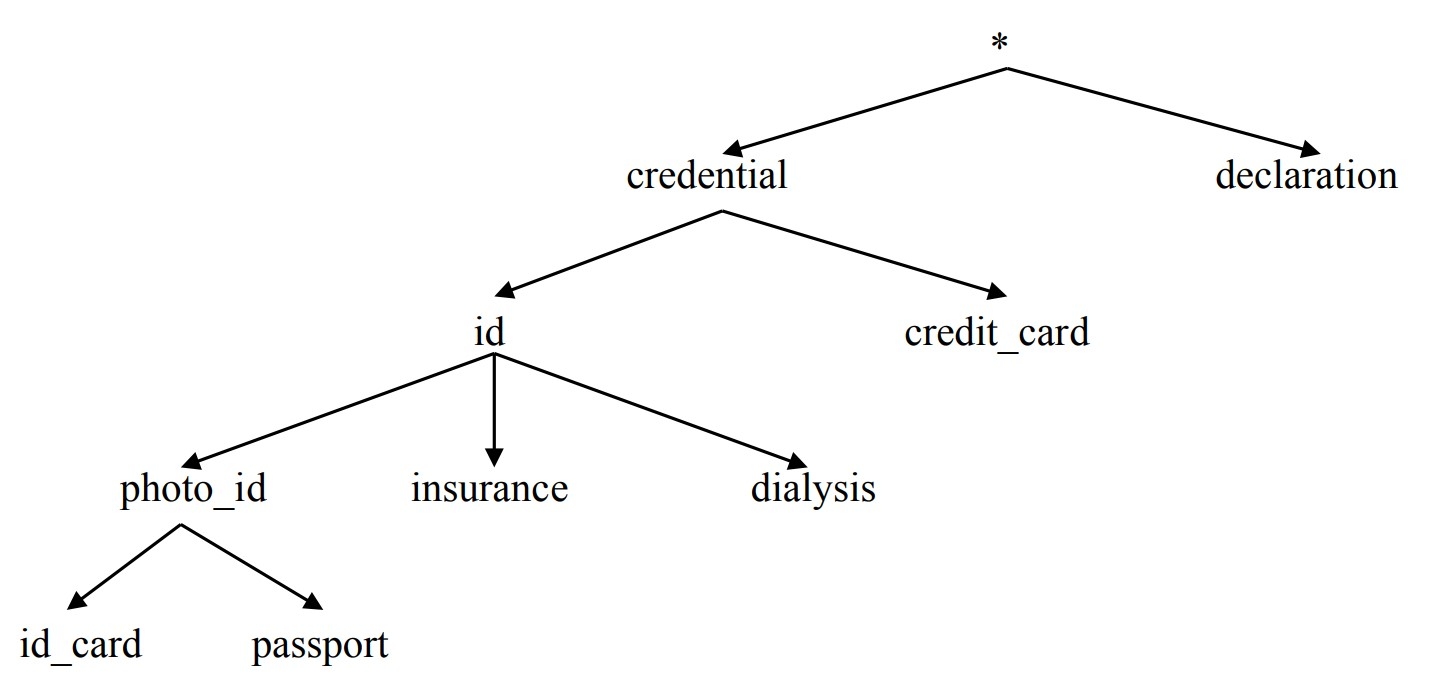
\includegraphics[width=0.8\textwidth]{paper_user-privacy-preferences/00_pref_credential_hierarchy.jpg}
    \caption{}
    \label{fig:00_pref_cred_hierarchy}
\end{figure}

La gerarchia è nota sia al client che al server. Il server tuttavia crea richieste di credential types in quanto non può conoscere le effettive credenziali possedute dal client\footnote{Inoltre client può avere più credenziali dello stesso tipo}.

\subsection{Atomicità Credenziali}
Le credenziali si distinguono in \textbf{atomiche} e \textbf{non-atomiche}.

$\\$
Le credenziali \textbf{atomiche} sono la tipologia più comune (vedi X.509) e possono essere rilasciato solo interamente.
Per questo anche attributi non richiesti vengono rivelati al server.

$\\$
Le credenziali \textbf{non-atomiche} permettono di limitare il rilascio di attributi rivelando selettivamente un subset degi attributi certificati dalla credenziale.

$\\$
Ovviamente le \textit{declaration} sono credenziali non-atomiche.


\subsubsection{Attributi}
Attributi nelle credenziali sono caratterizzati da:
\begin{itemize}
    \item Tipo
    \item Nome
    \item Valore
\end{itemize}
Essi possono essere \textit{credential-independent} e dipendere dal client ma non dalla credenziale, o \textit{credential-dependent} e dipendere da client e credenziale che la certifica.



\subsection{Policy di Disclosure}
Le policy lat server che regolano l'accesso sono definite sugli attributi e le credenziali fornite dall'utente, questo perchè il server considera solo la gerarchia di credenziali (conosciuta a priori anche dal server).

Una Access Control Policy (policy di controllo di accesso) è quindi una espressione booleana composta da condizioni \textit{ $ term_1 \, op \, term_2 $ } , dove \textit{op} è un operatore del tipo $<, >, =$ etc.

Un esempio di policy: \textit{ (type(c)= insurance) $\land$ (c.Company $\ne$ 'A') }





\subsection{Trust Negotiation}
L'interazione tra client e server mira a stabilire una relazione di fiducia (trust) tra le parti per permettere l'accesso al servizio.
Questa interazione si basa tipicamente sul rilascio di credenziali, spesso subordinato al rilascio di altre credenziali da parte della controparte.

Questa sequenza di scambi di credenziali è definita \textbf{strategia} e soddisfa le policy di server e client.

Alcune strategie adottate permettono il rilascio di credenziali solo se esiste una \textit{strategia di successo} (successful strategy) che garantisce l'accesso al servizio, mentre altre rilasciano credenziali appena sono richieste.

$\\$
Il fatto che esistano preferenze sul rilascio di credenziali, sia da parte del server che del client, comporta che le successful strategies non siano tutte equivalenti. 






\subsection{Client Privacy Preferences}
Per quanto riportato, è necessario fornire i client di un modello flessibile ed espressivo per rappresentare le preferenze di privacy.
Questo modello dovrebbe avere le seguenti caratteristiche:

\begin{itemize}
    \item \textbf{Specific di Preferenze a Grana Fine}: il modello deve supportare la definizione di preferenze per ogni attributo per ogni \textbf{istanza} di credenziale.
    \item \textbf{Ereditarietà delle Preferenze di Privacy}: se le istanze di credenziali sono numerose, il modello deve poter applicare sensibilità ai tipi astratti e così a tutte le istanze per cui non era stato specificato un livello di sensibilità.
    \item \textbf{Rel. d'Ordine Parziale e Operatore Composizione}: ci deve essere ordinamento parziale per determinare se una informazione è più o meno sensibile di un'altra. Deve esistere un operatore di composizione $\bigoplus$ che permette di calcolare il valore di sensibilità di un set di attributi/credenziali.
    \item \textbf{Associazioni Sensibili}: rilascio combinato di un set di attr./cred. risulta più o meno sensibile della somma dei rilasci singoli. Il modello deve comprendere anche questa definizione di preferenza.
    \item \textbf{Vincoli di Rilascio}: modello deve permettere di definire vincoli sul rilascio combinoato di parti del portfolio, per evitare o limitare il rilascio dell'associazione tra questi.
    \item \textbf{Context-Based Preferences}: preferenze dipendono dal contesto (rilasci certificato medico a una farmacia, non a un hotel).
    \item \textbf{History-based Preferences}: rilascio dipende da interazioni passate (se a server X ho rilasciato un set, uso sempre quello e non fornisco nuove cred.).
    \item \textbf{Prova di Possesso}: nuove tecnologie permettono di rilasciare prove di possesso di certificati e di soddisfazione requisiti di accesso. Risulta necessario poter specificare preferenze anche per queste prove (proof).
    \item \textbf{User-Friendly Preference Specification}: necessario fornire interfacce ai client, che possono non essere abituati a sistemi di controllo dell'accesso, per poter specificare facilmente le preferenze.
\end{itemize}




\subsection{Preferenze Privacy del Server}
Mentre la comunicazione della policy server completa favorisce la privacy del client, la comunicazione dei soli attributi coinvolti favorisce la privacy del server.

Ricordare che anche server ha un portfolio di credenziali e attributi oltre alle policy.

Il sistema lato server deve considerare:
\begin{itemize}
    \item \textbf{Disclosure Policy}: server deve poter decidere, a grana fine, come il rilascio policy dovrebbe essere regolato.
    \item \textbf{Comunicazione Policy}: necessario un meccanismo che trasforma la A.C.Policy in modo da proteggere privacy della policy e permettere al client di sapere cosa è richiesto.
    \item \textbf{Integrazione con Meccanismo Client}: Ci deve essere integrazione ra i sistemi lato server e lato client.
\end{itemize}




%%%   %%%   %%%
\section{Cost-Sensitive Trust Negotiation }
Sensibilità espressa con costo $w(c)$ associata ad ogni credenziale $c$ nel portfolio e con ogni policy di access control $p$.
$p$ viene definita come espressione booleana sulle credenziali della controparte, mentre i valori booleani delle credenziali $c$ sono espressi come $vero$ se già rivelati, $false$ altrimenti.

$\\$
Il costo di sensibilità, definito da utente, modella quanto l'owner ritiene sensibile il rilascio della credenziale e delle informazioni sensibili che certifica.

In fig. \ref{fig:pref_cost_example} un esempio di portfolio per client e server.
\begin{figure}[ht]
    \centering
    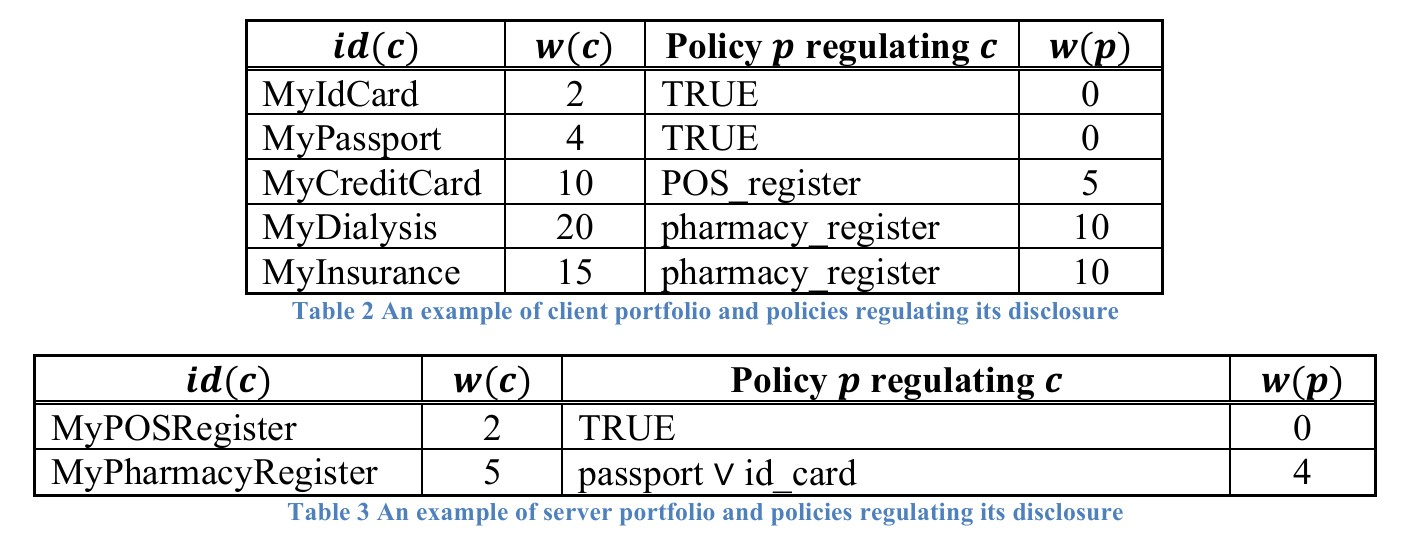
\includegraphics[width=0.8\linewidth]{paper_user-privacy-preferences/00_pref_cost_tab_example.jpg}
    \caption{Due esempi di portfolio con policy di rilascio}
    \label{fig:pref_cost_example}
\end{figure}

L'obbiettivo per client e serveer è quindi quello di minimizzare il costo di credenziali e policy scambiate \textbf{in una strategia di negoziazione che ha successo}.


\subsection{Minimizzare il Costo}
Il problema della minimizzazione del costo viene formulata come segue:

\begin{definition}[Problema del Minimo Costo di Sensibilità] $\\$
    Dati: \begin{itemize}
        \item $C_s$ set di credenziali e servizi server;
        \item $P_s$ set di policy server;
        \item $C_c$ set di credenziali client;
        \item $P_c$ set policy client;
        \item $w : \, C_s \cup P_s \cup C_c \cup P_c \, \rightarrow \mathbb{R}$ funzione costo;
        \item $s \in Cs$ il servizio richiesto.
    \end{itemize}
    Per minimizzare il costo in una successful strategy occorre trovare una sequenza di scambio tale che:
    \begin{enumerate}
        \item $s$ è rilasciato al client;
        \item ogni policy è soddisfatta prima del rilascio della corrispettiva credenziale;
        \item la somma dei costi è \textbf{minima}.
    \end{enumerate}
\end{definition}

\noindent Il problema è NP-difficile e con costo esponenziale nel numero di input(credenziali e policy).
Tuttavia due soluzioni euristiche (non ottimali) ottengono una buona soluzione con costo polinomiale. 
Queste considerano o meno il costo delle policy e sono brevemente\footnote{La completa descrizione degli algoritmi penso esuli dallo scope di questo riassunto} descritte qui di seguito:

\subsubsection{Senza Considerare Costo delle Policy}
Le policy non sono associate ad un costo, quindi possono essere pubblicate liberamente.

$\\$
Viene definito il DAG \textbf{policy graph $G(V,A,w)$} che modella le policy di rilascio delle credenziali sia lato server che lato client.

Un esempio del grafo è riportato in fig.\ref{fig:pref_policy_graph} che segue:

\begin{figure}[ht]
    \centering
    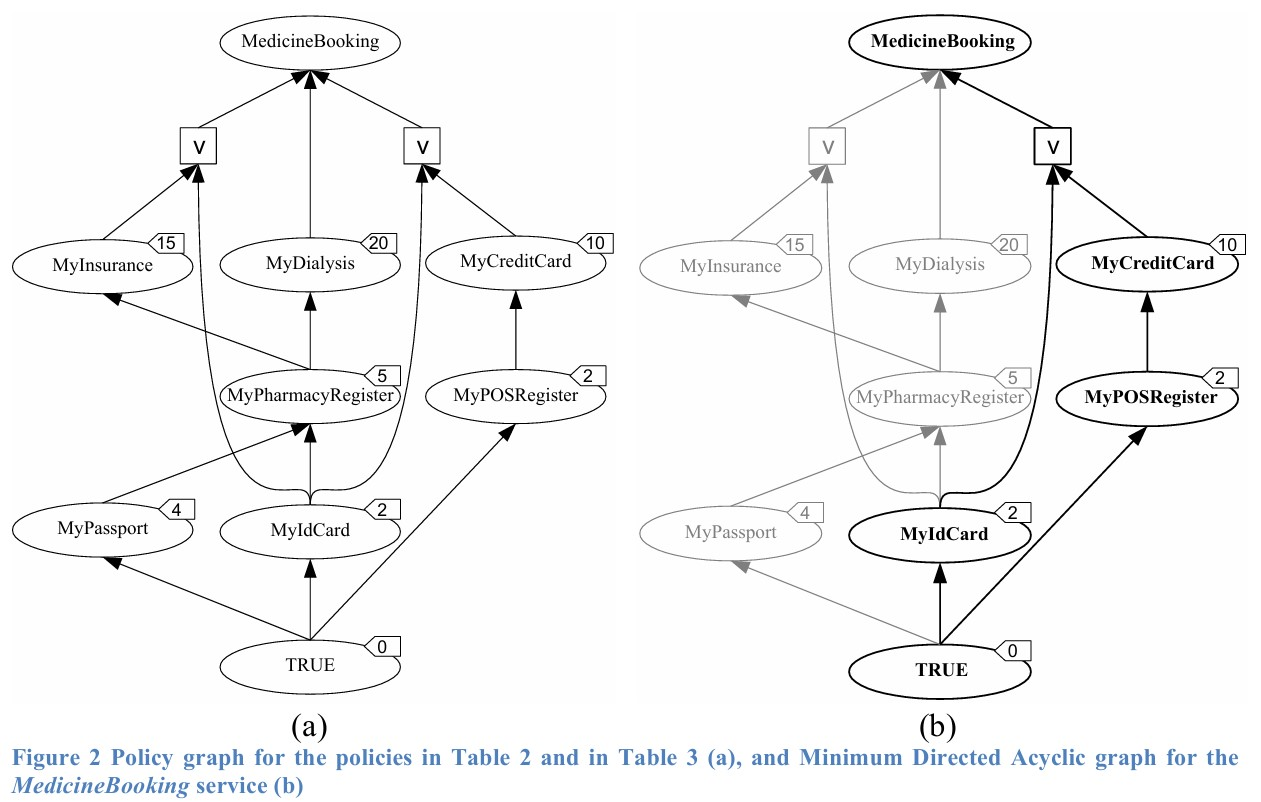
\includegraphics[width=0.8\linewidth]{paper_user-privacy-preferences/00_pref_policy_graph.jpg}
    \caption{Policy graph e suo DAG minimo.}
    \label{fig:pref_policy_graph}
\end{figure}

Il primo step riguarda sempre la disclosure delle policy, e ciò permette di costruire il grafo.

$\\$
Formalmente il problema si riduce pertanto al calcolo del DAG minimo.


\subsubsection{Considerando il Costo delle Policy}
Soluzione greedy che si divide in due step:
\begin{enumerate}
    \item Le parti adottano una \textit{eager strategy} che consiste nello scambiarsi i nomi delle credenziali e i relativi costi, previa soddisfazione della relativa policy, in modo da identificare una strategia che abbia successo.
    \item Applicazione della strategy trovata.
\end{enumerate}

In fig.\ref{fig:pref_policy_exchange} viene mostrato uno scambio per i portfolio mostrati precedentemente:

\begin{figure}[ht]
    \centering
    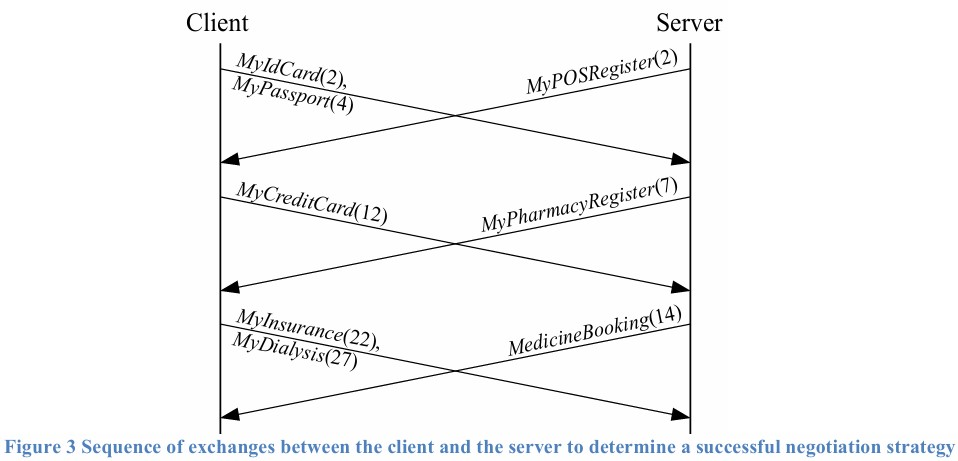
\includegraphics[width=0.8\linewidth]{paper_user-privacy-preferences/00_pref_policy_exchange.jpg}
    \caption{Scambio di credenziali tra le parti}
    \label{fig:pref_policy_exchange}
\end{figure}

\subsubsection{Problematiche Aperte}
Limitazioni dei due approcci: \begin{itemize}
    \item mancano le restrizioni sul rilascio delle policy;
    \item le parti non collaborano a minimizzare il costo a scapito della propria privacy (interessi delle parti);
    \item non supporta completamente la definizione desiderata espressa precedentemente.
\end{itemize}




%%%   %%%   %%%
\section{Point-Based Trust Management}
Questo sistema cambia il modello riguardante l'accesso alle risorse.
Viene associato un punteggio \texttt{ptr} ad ogni credenziale (in base al livello di affidabilità) ed una soglia \texttt{thr} di punti richiesti per ottenere accesso ad ogni servizio.

Il client deve quindi presentare un subset delle sue credenziali la cui somma dei punteggi supera la soglia richiesta dal server.

Allo stesso modo il client valuta il rilascio di ogni credenziale nel suo portfolio con un privacy score \texttt{ps}. Più è alto il ps, maggiore è la sensibilità della credenziale per il client\footnote{Cient rilascia credenziali con valori di \texttt{ps} minori.}.


$\\$
Infine, siccome le policy possono essere sensibili, il server non rilascia \texttt{thr} o il punteggio \texttt{pt} che associa alle credenziali, così come il client non rilascia i \texttt{ps}. Non conoscendo cosa è richiesto nasce quindi il \textit{Credential Selection Problem}.

\subsection{Credential Selection Problem}
Il problema consiste nel:
\begin{itemize}
    \item Trovare un subset di credenziali che soddisfa \texttt{thr}.
    \item Trovare un subset che sia minimo nella somma dei valori di \texttt{ps}.
\end{itemize}

E un problema NP-difficile.


\subsection{Dynamic Programming Algorithm}
Approccio che riscrive il problema in un \textit{knapsack problem}: vengono inseriti nel knapsack le credenziali che non verranno rilasciate.
Il knapsack ha capacità data dalla somma dei \texttt{pt} - il valore di soglia \texttt{thr} 


Tramite una matrice di appoggio vengono calcolate tutte le possibili modalità di riempimento del knapsack un elemento alla volta: ogni cella contiene il valore totale del knapsack per quello step di riempimento.
$\\$

Tuttavia \texttt{thr} e i \texttt{pt} vengono quindi comunicati.
Questo non è accettato nello scenario considerato, al che gli autori hanno proposto una soluzione di programmazione dinamica che permette alle parti di risolvere insieme il problema knapsack tramite crittografia homomorphica.


\subsubsection{Problematiche Aperte}
\begin{itemize}
    \item Comunicazione set di credenziali su cui basare lo scambio.
    \item \texttt{thr} non basta, server necessita di policy più espressive.
    \item Focus è sulla negoziazione e non sul management privacy preferences.
\end{itemize}





\section{Logical-Based Minimal Credential Disclosure}
Può non essere facile per un utente finale definire le preferenze con valori numerici come nelle soluzioni precedenti.
Inoltre valori numerici potrebbero imporre accidentalmente gerarchie come side effects.

Vengono quindi introdotti valori qualitativi per i valori di preferenza.
Le credenziali sono considerate singleton (certificano un solo attributo) e le policy server sono considerate note a tutti.

Utente deve infine scegliere una $strategy$ tra diverse opzioni, filtrate da tutte le strategie possibili tramite le preferenze utente. 

\subsection{Preferenze Qualitative}
La soluzione pratica sfrutta la composizione di Pareto\footnote{Qui vengono volutamente omessi i dettagli del funzionamento}.

$\\$
In sintesi, si rappresentano tutte le strategie di successo in una table che riporta il rilascio di ogni attributo.

Le preferenze sono invece espresse da foreste. Nodi a seguire di u arco direzionato sono più sensibili dei nodi alla partenza dell'arco.

Le strategie sono comparate attraverso la comparazione degli attributi secondo le relazioni di preferenza espresse. 


\subsubsection{Problematiche Aperte}
\begin{itemize}
    \item Richiede intervento utente per la scelta finale.
    \item Non considera le credenziali atomiche.
\end{itemize}






\section{Privacy Preferences in Credential-Based Interactions}
Soluzione che rispetta le \textit{desiderata} creando un portfolio modeling che permette di:
\begin{itemize}
    \item rappresentare credenziali atomiche e non;
    \item rappresentare dichiarazioni e attributi distinguendo chiaramente tra credential-dependent e credential-independent. 
\end{itemize}
Risulta più facile associare preferenze ad ogni credenziale e attributo.

\subsection{Rappresentazione Grafica del Portfolio}
Il portfolio viene rappresentato come un grafo bipartito $G(V_C \cup V_A , E_{CA})$ quale quello in figura fig.\ref{fig:pref_graph_portfolio}.


\begin{figure}[ht]
    \centering
    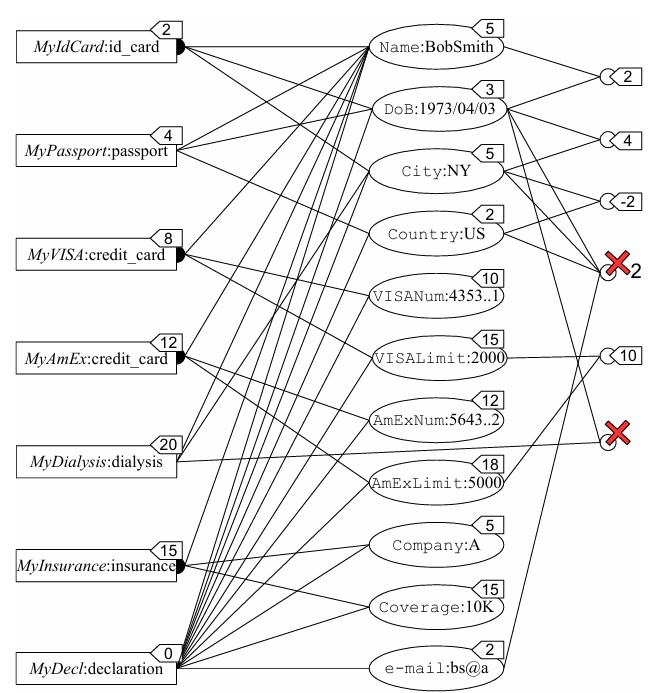
\includegraphics[width=0.8\linewidth]{paper_user-privacy-preferences/00_pref_graph_portfolio.jpg}
    \caption{Rappresentazione gafica del portfolio utente}
    \label{fig:pref_graph_portfolio}
\end{figure}

Il grafo ha a sinistra vertici rappresentanti le credenziali, a destra attributi, mentre gli archi associano gli attributi alle credenziali che li contengono.
Viene inoltre specificat atomicità delle credenziali con il simbolo nero accanto al vertice credenziale.
